\begin{frame}\begin{center}
		\LARGE\textbf{Identification}
\end{center}\end{frame}
%-------------------------------------------------------------------------------
%-------------------------------------------------------------------------------
\begin{frame}\textbf{Question}\vspace{0.3cm}

\begin{itemize}\setlength\itemsep{1em}
\item How do I know whether an RD design is appropriate for my context? When are the identification assumptions plausable or implausable?
\end{itemize}

\end{frame}
%-------------------------------------------------------------------------------
%-------------------------------------------------------------------------------
\begin{frame}\textbf{Answers}\vspace{0.3cm}

\begin{itemize}\setlength\itemsep{1em}
\item[$\times$] An RD design will be appropriate if it is plausible that all other unobservable factors are "continuously"  related to the assignment variable.

\item[\checkmark]  When there is a continuously distributed stochastic error component to the assignment variable - which can occur when optimizing agents do not have \textit{precise} control over the assignment variable - then the variation in the treatment will be as good as randomized in a neighborhood around the discontinuity threshold.
\end{itemize}

\end{frame}
%-------------------------------------------------------------------------------
%-------------------------------------------------------------------------------
\begin{frame}\textbf{Question}\vspace{0.3cm}

\begin{itemize}\setlength\itemsep{1em}
\item Is there any way I can test those assumptions?
\end{itemize}

\end{frame}
%-------------------------------------------------------------------------------
%-------------------------------------------------------------------------------
\begin{frame}\textbf{Answers}\vspace{0.3cm}

\begin{itemize}\setlength\itemsep{1em}
\item[$\times$] No, the continuity assumption is necessary so there are no tests for the validity of the design.

\item[\checkmark] Yes. As in randomized experiment, the distribution of observed baseline covariates should not change discontinuously around the threshold.

\end{itemize}

\end{frame}
%-------------------------------------------------------------------------------
%-------------------------------------------------------------------------------
\begin{frame}\textbf{Simplified setup}\vspace{0.3cm}

\begin{align*}
Y & = D \tau + W \delta_1 + U \\
D & = \Ind[X \geq c] \\
X & = W \delta_2 + V
\end{align*}

\begin{itemize}
\item $W$ is the vector of all predetermined and observable characteristics.
\end{itemize}

What are the source of heterogeneity in the outcome and assignment variable?

\end{frame}
%-------------------------------------------------------------------------------
%-------------------------------------------------------------------------------
\begin{frame}\textbf{Simplified setup}\vspace{0.3cm}

The setup for an RD design is more flexible than other estimation strategies.\vspace{0.3cm}

\begin{itemize}\setlength\itemsep{1em}
\item We allow for $W$ to be endogenously determined as long as it is determined prior to $V$.

\item We take no stance as to whether some elements $\delta_1$ and $\delta_2$ are zero (exclusion restrictions)

\item We make no assumptions about the correlations between $W$, $U$, and $V$.

\end{itemize}
\end{frame}
%-------------------------------------------------------------------------------
%-------------------------------------------------------------------------------
\begin{frame}

\begin{figure}[htp]\centering
\scalebox{0.60}{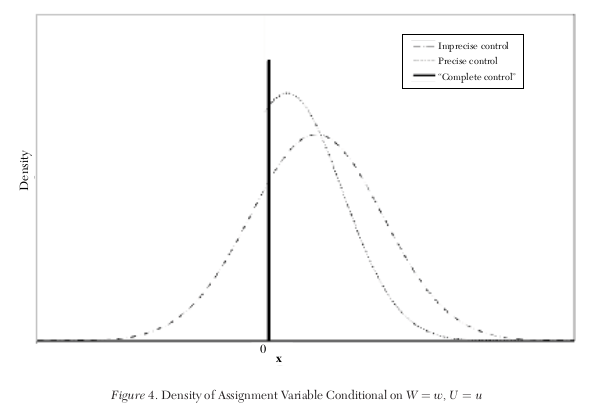
\includegraphics{material/fig-4}}
\end{figure}

\end{frame}
%-------------------------------------------------------------------------------
%-------------------------------------------------------------------------------
\begin{frame}\textbf{Local randomization}\vspace{0.3cm}

\textbf{Definition} We say individuals have imprecise control over $X$ when conditional on $W = w$ and $U = u$ the density of $V$ (and hence $X$) is continuous.

\end{frame}

%-------------------------------------------------------------------------------
%-------------------------------------------------------------------------------
\begin{frame}\textbf{Applying Baye's rule}\vspace{0.3cm}

\begin{align*}
& \Pr[W = w, U = u \mid X = x] \\
&\qquad\qquad = f(x \mid W = w, U = u) \quad\frac{\Pr[W = w, U = u]}{f(x)}
\end{align*}
\end{frame}
%-------------------------------------------------------------------------------
%-------------------------------------------------------------------------------
\begin{frame}\vspace{0.3cm}

\textbf{Local randomization} If individuals have imprecise control over $X$ as defined above, then $\Pr[W =w, U = u \mid X = x]$ is continuous in $x$: the treatment is "as good as" randomly assigned around the cutoff.\vspace{0.3cm}

$\Rightarrow$ the \textbf{behavioral} assumption of imprecise control of $X$ around the threshold has the \textbf{prediction} that treatment is locally randmized.

\end{frame}
%-------------------------------------------------------------------------------
%-------------------------------------------------------------------------------
\begin{frame}\textbf{Consequences}\vspace{0.3cm}

\begin{itemize}\setlength\itemsep{1em}
\item testing prediction that $\Pr[W =w, U = u \mid X = x]$ is continuous in $x$
\item irrelevance of including baseline covariates
\end{itemize}


\end{frame}
